\documentclass[10pt,a4paper]{book}
\usepackage[utf8]{inputenc}
\usepackage{amsmath}
\usepackage{amsfonts}
\usepackage{amssymb}
\usepackage{minted}
\definecolor{mygray}{gray}{0.9}
\usepackage{graphicx}
\usepackage{hyperref}
\usepackage{enumitem}
\author{Nicolò Fornari}
\title{Security testing}
\definecolor{mygray}{gray}{0.9}
\begin{document}
%\maketitle
\chapter{Assembly}
\section{Registers}
\textbf{What are registers for?}
\begin{itemize}[noitemsep,nolistsep]
\item Store instructions
\item Store result of operations
\item Manipulate data in them (shift registers)
\end{itemize}
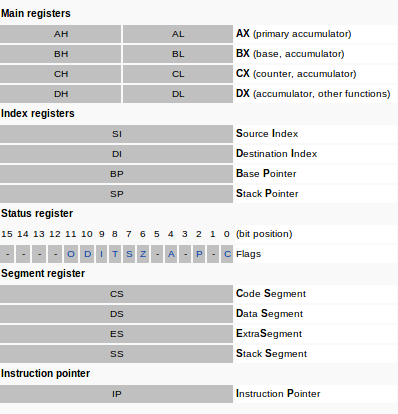
\includegraphics[scale=0.6]{registers.png}\\
\textbf{Why EAX,EBX,ECX?}
Registers AL,AH,BL,BH,CL,CH,DL,DH are of 16 bits each and can be used in pairs: AX, BX, CX, DX
\newpage
\section{Hello world}
\begin{minted}[
bgcolor=mygray,
]{as}
section .data
	hello:     db 'Hello world!',10    ; 
	helloLen:  equ \$-hello             ; Length of the 'Hello world'
	                                   ; (I'll explain soon)

section .text
	global _start

_start:
	mov eax,4            ; The system call for write (sys_write)
	mov ebx,1            ; File descriptor 1 - standard output
	mov ecx,hello        ; Put the offset of hello in ecx
	mov edx,helloLen     ; helloLen is a constant, so we don't need to say
	                     ;  mov edx,[helloLen] to get it's actual value
	int 80h              ; Call the kernel

	mov eax,1            ; The system call for exit (sys_exit)
	mov ebx,0            ; Exit with return code of 0 (no error)
	int 80h
\end{minted}
\\\\
Then in the terminal:\\\\
\begin{minted}[
bgcolor=mygray,
]{as}
nasm -f elf hello.asm
ld -m elf_i386 -s -o hello hello.o
\end{minted}
\\\\
Note that the elf\_i386 is necessary as we are writing 32 bit assembly code in a 64 bit architecture.
\newpage
\section{References}
\begin{enumerate}
\item \url{https://www.quora.com/What-is-an-intuitive-explanation-of-how-CPU-registers-work}
\item \url{http://stackoverflow.com/questions/2545192/what-does-x-mean-in-eax-ebx-ecx-in-assembly}
\item \url{http://docs.cs.up.ac.za/programming/asm/derick_tut/}
\end{enumerate}

\end{document}
